\documentclass[12pt]{report}

\usepackage[a4paper,
			inner = 35mm,
			outer = 25mm,
			top = 25mm,
			bottom = 25mm]{geometry}
\usepackage{lmodern}
\usepackage[magyar]{babel}
\usepackage[utf8]{inputenc}
\usepackage[T1]{fontenc}
\usepackage[hidelinks]{hyperref}
\usepackage{graphicx}
\usepackage{amssymb}
\usepackage{setspace}
\usepackage[nottoc,numbib]{tocbibind}
\usepackage{amsthm}
\usepackage{minted}
\usepackage{mdframed}
\usepackage{etoolbox}
\usepackage{svg}



% \setcounter{secnumdepth}{3}
\onehalfspacing

\newtheorem{mydef}{Definició}
\newtheorem{mytetel}{Tétel}
\newtheorem{mylemma}{Lemma}

\BeforeBeginEnvironment{minted}{\begin{mdframed}[backgroundcolor=bg, hidealllines=true]}
\AfterEndEnvironment{minted}{\end{mdframed}}

\newcommand{\cmd}[1]{\colorbox{gray!10}{\strut #1}}

\definecolor{bg}{rgb}{0.95,0.95,0.95}
\newminted[mintedJson]{js}{breaklines, breaksymbolleft=\quad}
\newminted[mintedBash]{bash}{breaklines, breaksymbolleft=\quad}



\begin{document}

\begin{titlepage}
	\begin{center}
		\vspace*{1cm}
		
		\textbf{\LARGE 
			Forgalom igény tudatos hálózat tervezés minimális torlódással és úthosszal
		}
	
	
		\vspace{0.5cm}
	
		\textbf{\normalsize Tudáskezelő rendszerek II. labor összefoglaló}
		
		\vfill
		
		\Large Szecsődi Imre
		
		\vspace{2.8cm}
		
		\the\year
		
	\end{center}
\end{titlepage}

\tableofcontents
	
\chapter{Bevezetés}

A labor munka a Demand-Aware Network Design with Minimal Congestion and Route Lengths \cite{avin_demand-aware_nodate} cikk alapján készült.

\section{Motiváció}

\begin{itemize}
	\item A technika előrehaladásával egyre nagyobb lett a feldolgozandó adatok mennyisége
	\item Adattárházakban a szerverek közötti kommunikáció is ezáltal megnövekedett
	\item A jelenlegi hálózatok a legrosszabb esetre vannak tervezve, azaz, hogy majdnem teljes sávszélességű, kétirányú kapcsolat álljon fent bármelyik két szerver között
	\item A valós kommunikáció nem ezt a sémát követi, hanem túlnyomó részt megadott párok között történik a legtöbb kommunikáció
\end{itemize}

Microsoft Research ProjecToR \cite{ghobadi_projector:_2016}.

\begin{itemize}
	\item Nézzünk meg pár valós példát, Microsoft adattárházában  250 ezer szervert 5 production klaszterben elosztva
\end{itemize}

\subsection{Hálózat tervezési stratégiák}

\begin{center}
	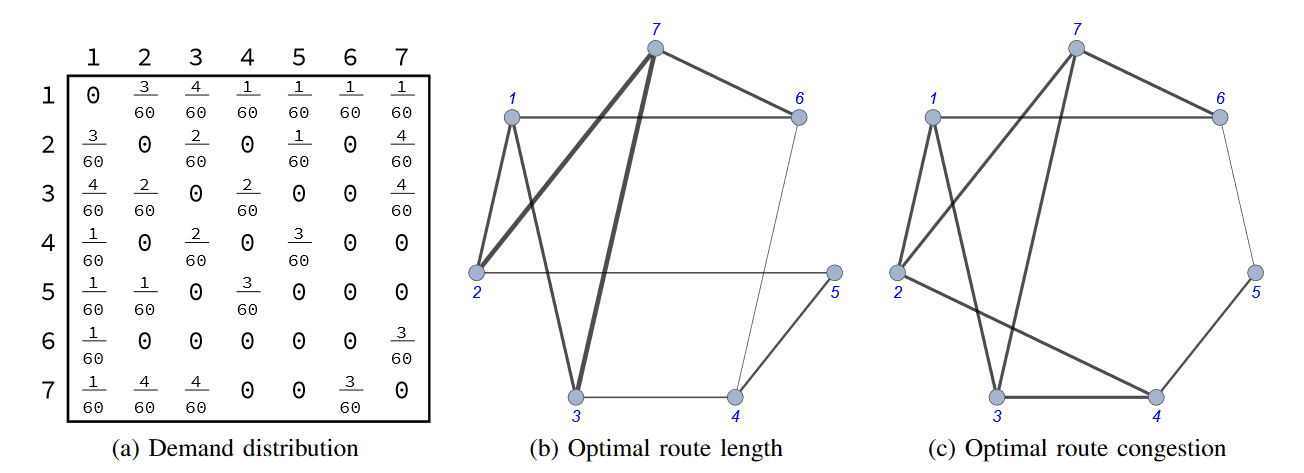
\includegraphics[width=14cm]{pictures/example.png}
\end{center}

\begin{itemize}
	\item A technika fejlődésével elérhetővé váltak eszközök arra, hogy egy adott hálózatot újra konfiguráljunk, attól függően milyen terhelés éri
	\begin{itemize}
		\item pl, korábbi kommunikációs minták alapján
	\end{itemize}
	\item Két fő optimalizációs lehetőség van, legyen rövid az út (a) vagy legyen minimális a torlódás (b)
	\item A cikk bemutat egy módszert arra, hogy lehet mindkettőre majdnem optimális megoldást adni egyszerre (c)
\end{itemize}



\subsection{Adattárházak hálózati felépítése}

\begin{center}
	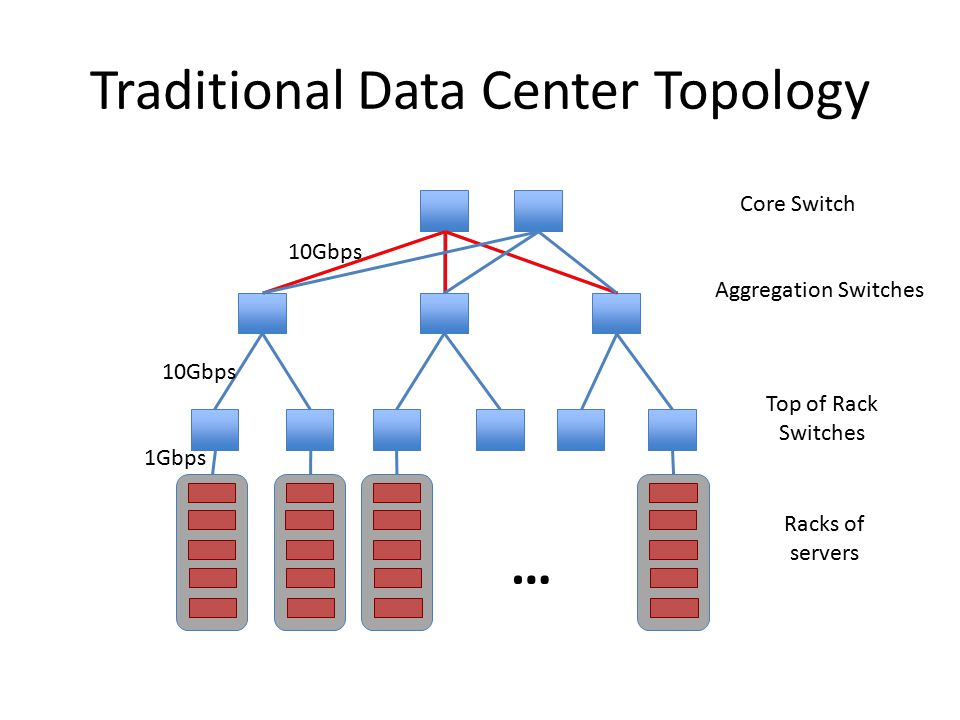
\includegraphics[width=0.7\linewidth]{pictures/Traditional+Data+Center+Topology.jpg}
\end{center}

\begin{itemize}
	\item Core switch
	\item Aggregation Swtiches
	\item Top of Rack Switches
	\item In-Rack Switches
\end{itemize}

\subsection{Újrakonfigurálás megvalósítása}

\begin{itemize}
	\item Átlag hálózatok statikusan vannak konfigurálva, nem  sok lehetőséget adva annak, hogy változtassunk 
	\begin{itemize}
		\item pl. Ethernet switchek
	\end{itemize}
	\item Optikai switchek már újra tudják konfigurálni magukat, de ezek "lassúak"
	\item Microsoft Research - ProjecToR\cite{ghobadi_projector:_2016}, lézer segítségével kiváltani az optikai swticheket, \ref{projector-fig} ábrán látható a maga az eszköz
	\begin{itemize}
		\item 12 $\mu s$ váltás idő ( 2500x gyorsabb mint egy optikai hálózati switch)
	\end{itemize}
	
	\begin{figure}[h]
		\centering
		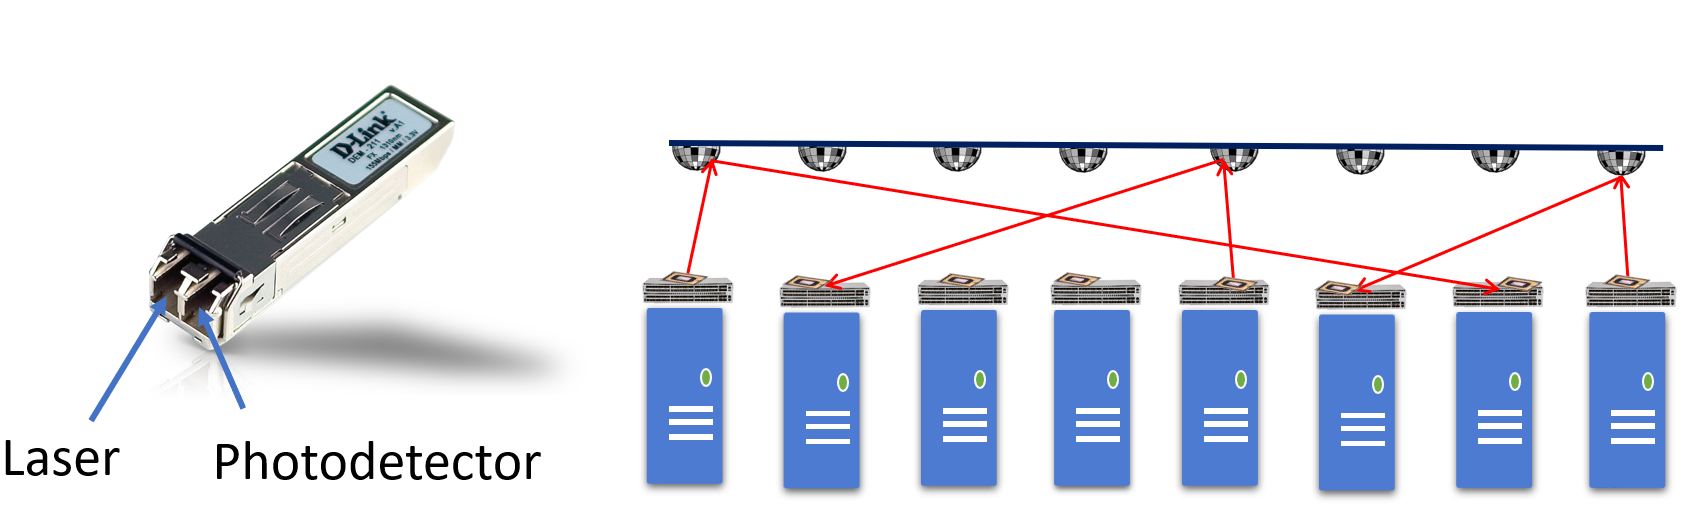
\includegraphics[width=0.9\linewidth]{pictures/laserswitch.png}
		\caption{ProjecToR}\label{projector-fig}
	\end{figure}
	
	
\end{itemize}

\section{Labor célja}

A labor célja a cikkben\cite{avin_demand-aware_nodate} bemutatott algoritmus implementálása, és annak alkalmazása különböző véletlenszerűen generált gráfokra. 
A kapott eredményeket össze lehet hasonlítani a megadott elméleti korlátokkal.

\section{Laborban megvalósított munka}

A labor ideje alatt elkészült egy keretrendszer, ami segítségével tesztelhető a szerzők által felvázolt algoritmus. 
A keretrendszer Python \cite{noauthor_python_nodate} nyelven íródott.
Egy véletlen gráfok generálására egy külső csomag lett használva \cite{noauthor_networkx_nodate}

\chapter{Modell}

\section{Forgalom igény tudatos hálózat tervezés probléma}

\begin{itemize}
	\item Vegyünk egy hálózatot meghatározott számú csomóponttal
	\item A hálózathoz tartozik egy demand mátrix, ami leírja a valószínűségét annak, hogy $i$ forrásból mekkora eséllyel lesz adat küldve $j$ célba
	\item A cél, hogy ezen adatból egy olyan hálózati séma készítése, ami kis torlódást és rövid utakat eredményez, ez mellett még skálázható is
\end{itemize}

\section{Formális felírás}

\begin{itemize}
	\item Adott $N$ darab csúcspont  $V = \{1, ..., N\}$, és egy kommunikációs séma $M_D$ ami egy $N\times N$ mátrix
	\item A mátrix $(i, j)$ eleméhez tartozik egy $p(i, j)$ valószínűség, ahol $i$ a forrás csomópont és $j$ a cél
	\item A bemeneti mátrix ábrázolható egy irányított
	$G_D$ gráfban, ahol az élsúlyok a két pont közötti kommunikációs valószínűség
	\item Az algoritmus feltétele, hogy a mátrix ritka legyen
	\item Egy $N$ hálózatra a torlódást és az úthosszt útválasztási sémával fogjuk definiálni
	\item Egy útválasztási séma az $N$ hálózatra $\Gamma(N)$, ami $\Gamma_{uv}$ utak halmaza, ahol $(u, v)$ párok különböző utakat jelölnek
	\item $\Gamma_{uv}$ egy útsorozat, ami összeköti az $u$ pontot $v$ ponttal
\end{itemize}

\subsection{Torlódás}

\begin{mydef}
	A torlódást egy \(\Gamma(N)\) útválasztási sémán a \(D\) demand mátrix segítségével írjuk fel: \[C(D, \Gamma(N)) = \max_{e \in \Gamma(N)}  \sum_{e \in \Gamma(uv)} p(u,v) \]
\end{mydef}

\subsection{Úthossz}

\begin{mydef}
	Az átlag súlyozott úthosszt egy \(\Gamma(N)\) útválasztási sémán a \(D\) demand mátrix segítségével írjuk fel: \[L(D, \Gamma(N)) = \sum_{(u,v) \in D}  p(u,v)  \cdot d_{\Gamma(N)}(u, v) \] ahol a \(d_{\Gamma(N)}(u, v)\) az útvonal hosszát jelöli
\end{mydef}

\subsection{Skálázhatóság}

\begin{itemize}
	\item A hálózatot skálázhatóra kell tervezni, ezért meghatározunk egy \(\Delta\) konstans fokszámot, ami a maximális csatlakozások számát fogja meghatározni egy adott csomóponthoz
	\item \(N_\Delta\) jelölje az összes \(\Delta\) fokszámú gráfot, és elváruk, hogy \(N \in N_\Delta\)
\end{itemize}

\subsection{Optimális torlódás}

Az optimális torlódást egy  hálózatra, úgy határozzuk meg, hogy a csak a torlódást vesszük figyelembe számításkor \[C^*(D, \Delta) = \min_{N \in N_\Delta, \Gamma(N)} C(D, \Gamma(N))\]

\subsection{Optimális úthossz}

Az optimális úthosszt egy  hálózatra, úgy határozzuk meg, hogy a csak az úthosszt vesszük figyelembe számításkor \[L^*(D, \Delta) = \min_{N \in N_\Delta, \Gamma(N)} L(D, \Gamma(N))\]

\section{cl-DAN hálózat tervezése}
	
\begin{mydef}
	Adott egy \(D\) demand mátrix, és egy \(\Delta\) maximális fokszám, az \((\alpha, \beta)\)-cl-DAN hálózat tervezési probléma:
	\begin{itemize}
		\item Hogy tervezzünk egy olyan \(N \in N_\Delta\) hálózatot, és egy hozzá tartozó \(\Gamma(N)\) útválasztási sémát, ami közel optimális torlódásra és úthosszra is
	\end{itemize}

	Az algoritmus egy felső korlátot tud adni arra, hogy mennyivel fog eltérni a megoldás az optimálistól.
	\begin{itemize}
		\item Torlódásra: \(C(D, \Gamma(N)) \le \alpha \cdot C^*(D, \Delta) + \alpha'\)
		\item Úthosszra: \(L(D, \Gamma(N)) \le \beta \cdot L^*(D, \Delta) + \beta'\)
	\end{itemize}
	Az alfa vessző és béta vesszők olyan tényezők aki amik függetlenek a problémától
\end{mydef}

\section{EgoTree}

\begin{itemize}
	\item Az Egofa egy torlódásra és úthosszra optimalizált fa hálózat egy csomópontra nézve
	\item Az Egotree-t definiáljuk a következő módon, 
	
	\(EgoTree(s, \bar{p}, \Delta) \):
	\begin{itemize}
		\item \(s\) a forrás csomópont
		\item \(\bar{p}\) a szomszédainak eloszlásai
		\item \(\Delta\) fokszám
	\end{itemize}
	\item Ez közel optimális megoldást ad torlódásra és úthosszra
\end{itemize}

\begin{mytetel}
	Adott egy  \(\bar{p}\) frekvencia eloszlás az \(s\) forrás ponthoz, és adott egy \(\Delta\) fokszám, ekkor az \(EgoTree(s, \bar{p}, \Delta)\) egy \((\alpha, \beta)\)-cl-DAN a következő paraméterekkel:
	\begin{itemize}
		\item \(\alpha = \frac{4}{3}\)
		\item \(\beta = log^2(\Delta + 1)\)
	\end{itemize}
\end{mytetel}

\section{\(EgoTree(s, \bar{p}, \Delta)\) algoritmus}

\begin{enumerate}
	\item \(s\) a gyökér elem, \(\Delta\) fokszámmal, üres fa
	\item Rendezzük sorba \(\bar{p} = \{p1, p2, ..., p_k\}\) valószínűségeket csökkenő sorrendben
	\item Kezdjük rárakni a fára a csomópontokat, a gyökér elemre legfeljebb \(\Delta\) levél kerülhet
	\item Mikor elértük a \(\Delta\) levelet, a következő csomópontokat mindig a legkisebb összesített súlyú levélre kapcsolok rá, itt már legfeljebb két levele lehet minden fának
\end{enumerate}

\subsection{Algoritmus elemzése}

\begin{itemize}
	\item A kapott eredményben látható, hogy a maximális torlódás a legnagyobb súlyú élen van
	\item Minimalizálni ezt, lényegében egy időzítés probléma, hogy osszuk ki a munkákat \(\Delta\) processzornak, hogy minden leghamarabb kész legyen
	\item Erre az optimális algoritmus NP-nehéz, de van közelítő módszer
\end{itemize}

\subsection{Longest Processing Time (LPT)}

\begin{itemize}
	\item Először sorba rendezzük a feladatokat hossz szerint csökkenő sorrendben
	\item Ha van szabad processzor, akkor ahhoz rendeli a leghosszabb munkát
	\item Ha nincs akkor ahhoz a processzorhoz rendeli, ahol a legkevesebb ideig tart a munka
\end{itemize}
\begin{mytetel}
	Legyen \(\omega_L\) a maximum idő, mielőtt egy processzor befejezi az összes munkát a mohó LPT algoritmus szerint, és \(\omega_0\) az optimális, ekkor \[\frac{\omega_L}{\omega_0} \le \frac{4}{3} - \frac{1}{3\Delta}\]
\end{mytetel}

Ez az algoritmus polinom időben lefut

\begin{mylemma}
	Az \(EgoTree(s, \bar{p}, \Delta)\) ad egy \(\frac{4}{3}\) szorzóval nagyobb közelítést a minimális torlódásra az optimális \(\Delta\) fokú fához képest, ami kiszolgál \(\bar{p}\) frekvencia eloszlást egy adott \(s\) forrás csomópontra
\end{mylemma}

\begin{mylemma}
	Az \(EgoTree(s, \bar{p}, \Delta)\) ad egy \(log^2(\Delta + 1)\) szorzóval nagyobb közelítést a minimális úthosszra az optimális \(\Delta\) fokú fához képest, ami kiszolgál \(\bar{p}\) frekvencia eloszlást egy adott \(s\) forrás csomópontra
\end{mylemma}

\section{cl-DAN algoritmus}

\begin{mytetel}
	Legyen \(D\) egy szimmetrikus kommunikáció kéréseloszlás , ahol az átlag csúcs fokszáma \(\rho\), (azaz az élek száma \(\rho \cdot \frac{n}{2}\). Ekkor a maximum fokszám \(\Delta = 12\rho\), ehhez lehetséges generálni egy \((\alpha, \beta)\)-cl-DAN hálózatot, ahol:
	\begin{itemize}
		\item \(\alpha = 1 + (\frac{8}{9})\Delta\)
		\item \(\beta = 1 + 4log^2(\Delta + 1)\)
	\end{itemize}
\end{mytetel}
Konstans \(\rho\) esetén ez konstans közelítést ad a minimális torlódásra és az optimális úthosszra

\begin{enumerate}
	\item Felosszuk a hálózat csúcsait két halmazra, \(H\) - magas és \(L\) - alacsony fokszámúakra fele-fele arányban
	\begin{itemize}
		\item Az alacsony fokszámú csúcsok fokszáma legfeljebb \(2\rho\)
	\end{itemize}
	\item Megkeressük az összes olyan \((u, v)\) élt, ahol \(u\) és \(v\) is a magas fokszámú halmazba tartozik
	\item Az ilyen éleket a gráfban kiegészítjük egy segítő csomóponttal, \(l \in L\), az eredeti csomópontok között megszüntetjük az élt, és felveszünk két új élt \((u, l)\) és \((v, l)\)
	\begin{itemize}
		\item Minden segítő \(l\) csúcs választásakor egy még nem felhasználtat válasszunk az \(L\) halmazból
	\end{itemize}
	\item Meghatározunk egy mátrixot, ami első lépésben az eredeti
	\begin{itemize}
		\item Ahol segítő csomópontot vettünk fel, ott az útvonal hosszúhoz hozzá kell még adni az \(l\)-el való áthaladást is, és törölni kell az eredeti pontok közti élt
		\item Ezután elkészítjük a magas halmaz csúcsaira a \(T_u\) fát, ahol a valószínűségeket a mátrixból kiolvassuk, \(\Delta = 12\rho\) fokszámmal, ez közel optimális megoldást ad mindkét fel
	\end{itemize}
	\item Mivel \(u\) és \(v\) pontok közt egy \(l\) segítő csomópont van használva ezért \(T_u\) és \(T_v\) módosításra szorul. Alakítsuk át először \(T_u\)-t \(T'_u\)-ra
	\begin{itemize}
		\item Ha \(l \notin T_u\), \((p(u, l) = 0)\), akkor \(l\) átveszi \(v\) helyét \(T'_u\)-ban
		\item Ha \(l \in T_u\), \((p(u, l) > 0)\), akkor két lehetőségünk van:
		\begin{itemize}
			\item Ha \((p(u, l) > (p(u, v))\), akkor töröljük \(v\)-t a fából
			\item Ha \((p(u, l) \le (p(u, v))\), akkor \(l\) átveszi \(v\) helyét \(T'_u\)-ban
		\end{itemize}
		\item \(T'_v\) hasonlóan számítjuk ki, ezzel garantálva, hogy \(T'_u\) és \(T'_v\) közötti kommunikáció az \(l\) csomóponton keresztül fog áthaladni
	\end{itemize}
	\item Konstruáljuk meg az új N hálózatot, vegyük az előbb készített egofákat és vegyük az uniójukat, azaz húzzuk be az összes olyan élet amik szerepeltek a fákban
	\begin{itemize}
		\item     De mivel nem csak magas fokú csomópontok közt történhetett adatforgalom, ezért még vegyük hozzá az N hálózathoz azokat az éleket is, ahol mindkét csomópont alacsony fokszámú volt
	\end{itemize}
\end{enumerate}

\chapter{Megvalósítás}

\section{Keretrendszer}

A keretrendszer Python 3 nyelven íródott, és a Networkx külső csomag volt használva a véletlen gráfok generálására.
A példakód megtalálható futtatható hagyományos Python programként és Jupyter notebookban.  

\section{Adatszerkezetek}

A modell alapját pár egyszerű alaptípus adja. Ezek rendre a következők:
\begin{itemize}
	\item \textbf{Vertex} - az általános gráf csúcspont
	\item \textbf{Node} - az \textit{Egófák} készítésekor használt csomópontok amik tartalmazzák a valószínűségét annak, hogy a forrás csomópont mekkora valószínűséggel fog kommunikálni a másik \textit{Node} csomóponttal
	\item \textbf{Edge} - az gráf csomópontjait reprezentáló szakasz, ami \textit{Vertexet} vár paraméterként, és tárolja a valószínűséget, hasonlóan mint a \textit{Node}
	\item \textbf{Tree} - ami adja az alapját majd a útvonal tervezési sémának. A fának két fajtája lehet:
	\begin{itemize}
		\item \textbf{BinTree} - a kettő fokú fa
		\item \textbf{EgoTree} - a $\Delta$ fokú fa, ahol a gyökérnek legfeljebb $\Delta$ levele lehet, és a levelek pedig \textit{BinTree} típúsuak.
	\end{itemize}
	
\end{itemize}
	
\section{Modell}

A \textbf{Network} osztály valósítja meg az algoritmust, bemenete egy konfiguráció, kimenete egy útválasztási séma.
Az útválasztási séma mellett még metaadatként ki van számolva az átlag súlyozott úthossz és a torlódás az adott hálózatra.

Bementi konfigurációt többféle módon lehet megadni attól függően milyen gráfot akarunk használni. 
Lehetőség van kézileg megadni a demand mátrixot vagy generálhatunk kétféle véletlen gráfot.
Véletlen gráfok amit tud generálni a program:
\begin{itemize}
	\item Erdős-Rényi gráf
	\item Barabási-Albert gráf
\end{itemize}

Egy minta konfiguráció, ami tartalmaz példát mind három esetre:


\begin{mintedJson}
{
  "config": [ {
	"graph": "erdos-renyi",
	"vertex_num": 11,
	"dan": null,
	"constant": 3
  }, {
	"graph": "barabasi-albert",
	"vertex_num": 11,
	"dan": 3,
	"m": 4
  }, {
	"graph": "manual",
	"vertex_num": null,
	"dan": 3,
	"demand": [
		[0, 3, 4, 1, 1, 1, 1],
		[3, 0, 2, 0, 1, 0, 4],
		[4, 2, 0, 2, 0, 0, 4],
		[1, 0, 2, 0, 3, 0, 0],
		[1, 1, 0, 3, 0, 0, 0],
		[1, 0, 0, 0, 0, 0, 3],
		[1, 4, 4, 0, 0, 3, 0]]	
	} ]
}
\end{mintedJson}

\section{Kimenet}

Az program kimenete, az algoritmus által kiszámolt metrikák, átlag súlyozott úthossz és torlódás. 
Ha a rajzolás opció be van kapcsolva, akkor a kiindulási hálózat, az egófák és az új hálózat választási séma ki lesz rajzolva.

\begin{figure}[h]
	\begin{center}
		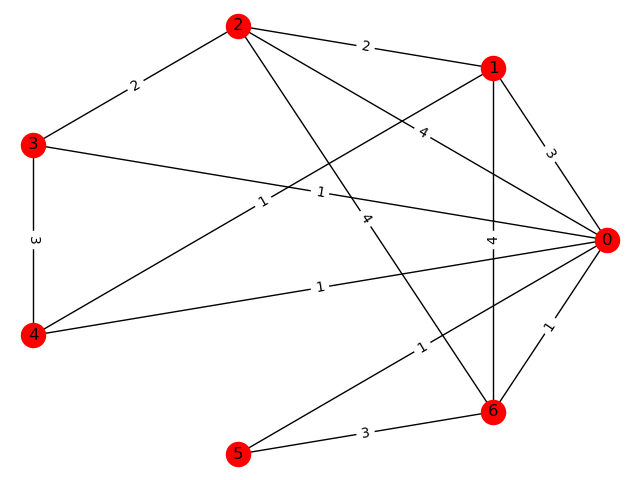
\includegraphics[width=0.49\linewidth]{pictures/starting_network.png}
		\caption{Kiindulási hálózat}
	\end{center}
\end{figure}

\begin{figure}[h]
	\begin{center}
		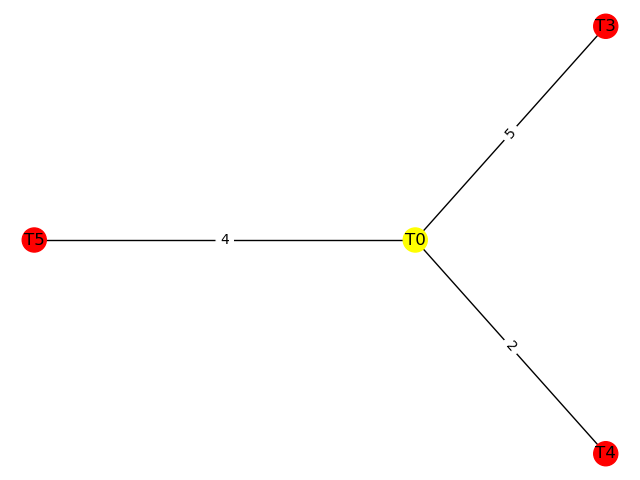
\includegraphics[width=0.40\linewidth]{pictures/egotree1.png}
		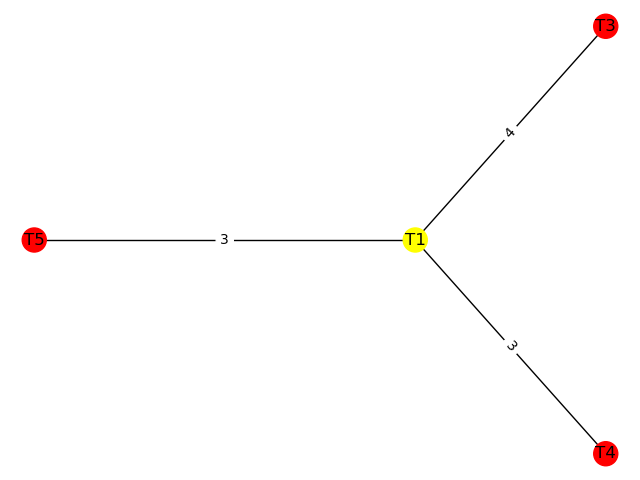
\includegraphics[width=0.40\linewidth]{pictures/egotree2.png}
		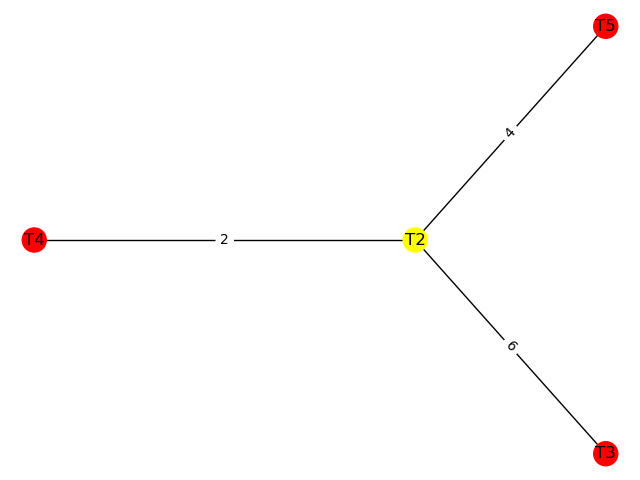
\includegraphics[width=0.40\linewidth]{pictures/egotree3.png}
		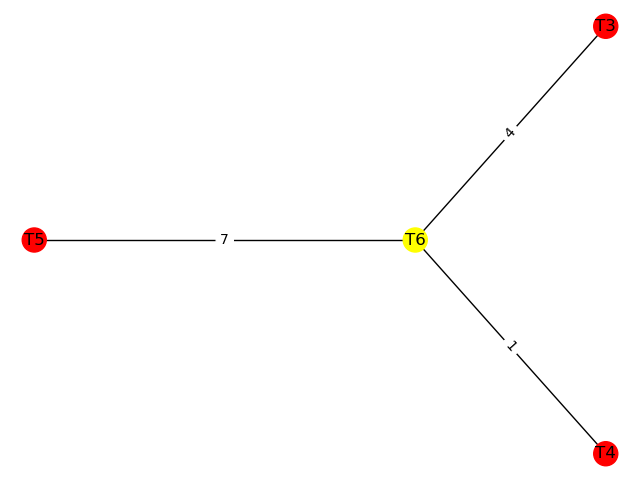
\includegraphics[width=0.40\linewidth]{pictures/egotree4.png}
		\caption{Egófák}
	\end{center}
\end{figure}

\begin{figure}[h]
	\begin{center}
		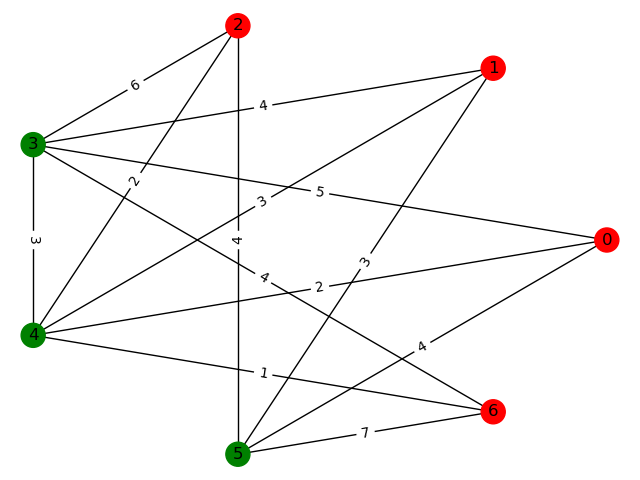
\includegraphics[width=0.49\linewidth]{pictures/new_network.png}
		\caption{Új hálózat}
	\end{center}
\end{figure}

\chapter{Teszt eredmények}

\begin{figure}[h]
	\begin{center}
		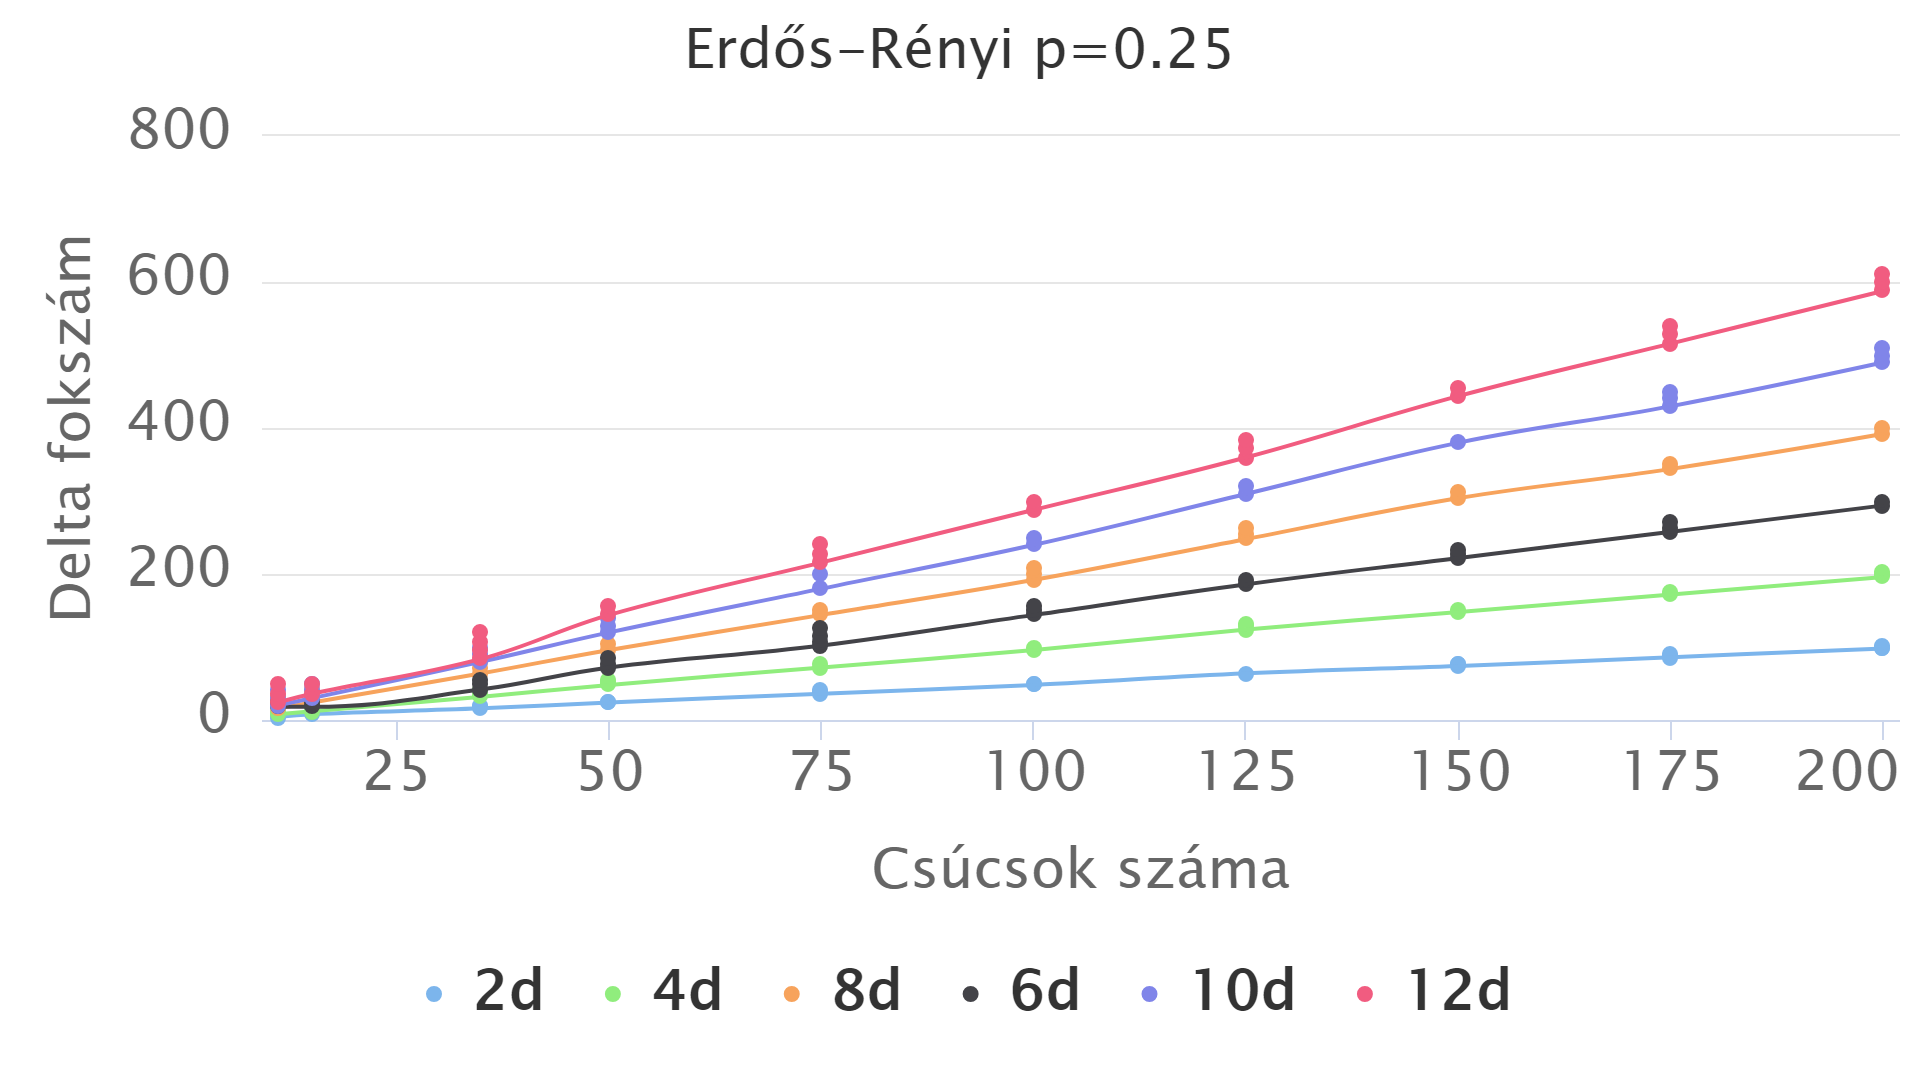
\includegraphics[width=0.49\linewidth]{pictures/constant_dan_ratio25_delta.png}
		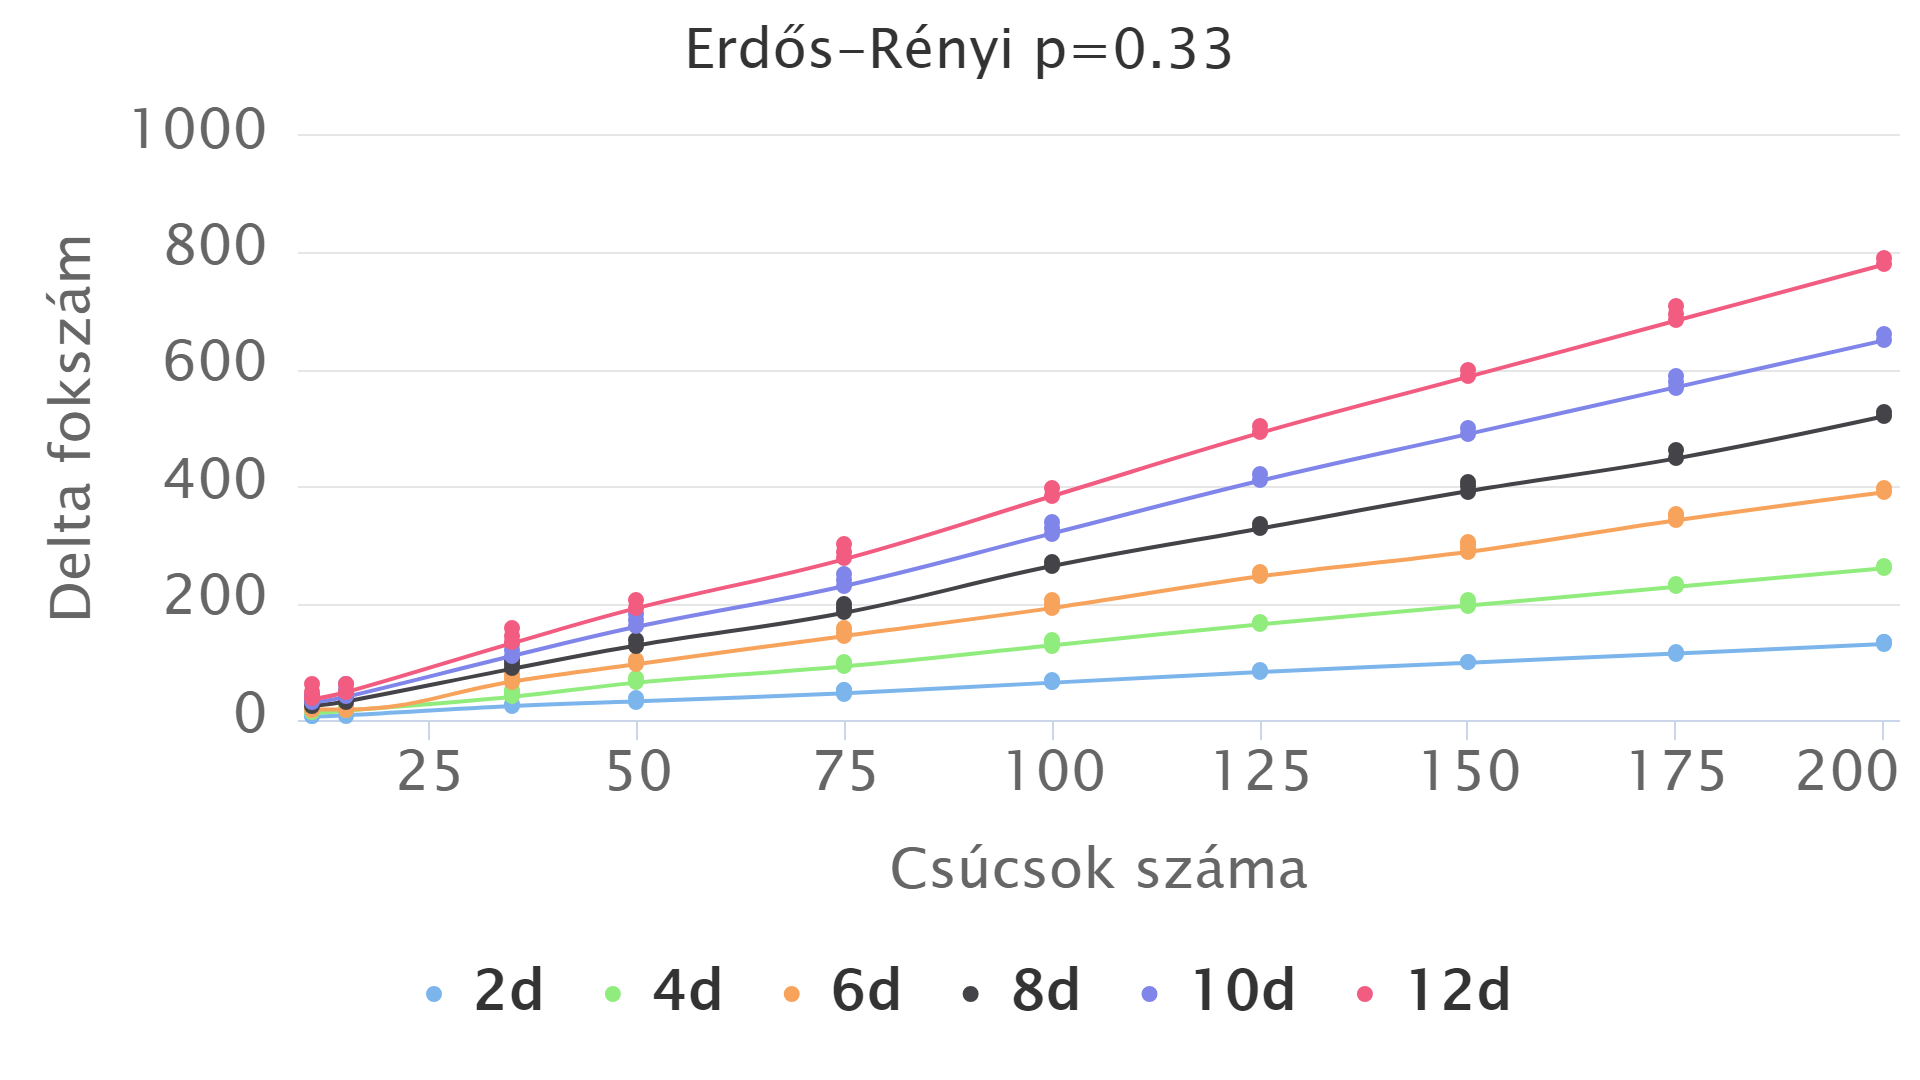
\includegraphics[width=0.49\linewidth]{pictures/constant_dan_ratio33_delta.png}		
		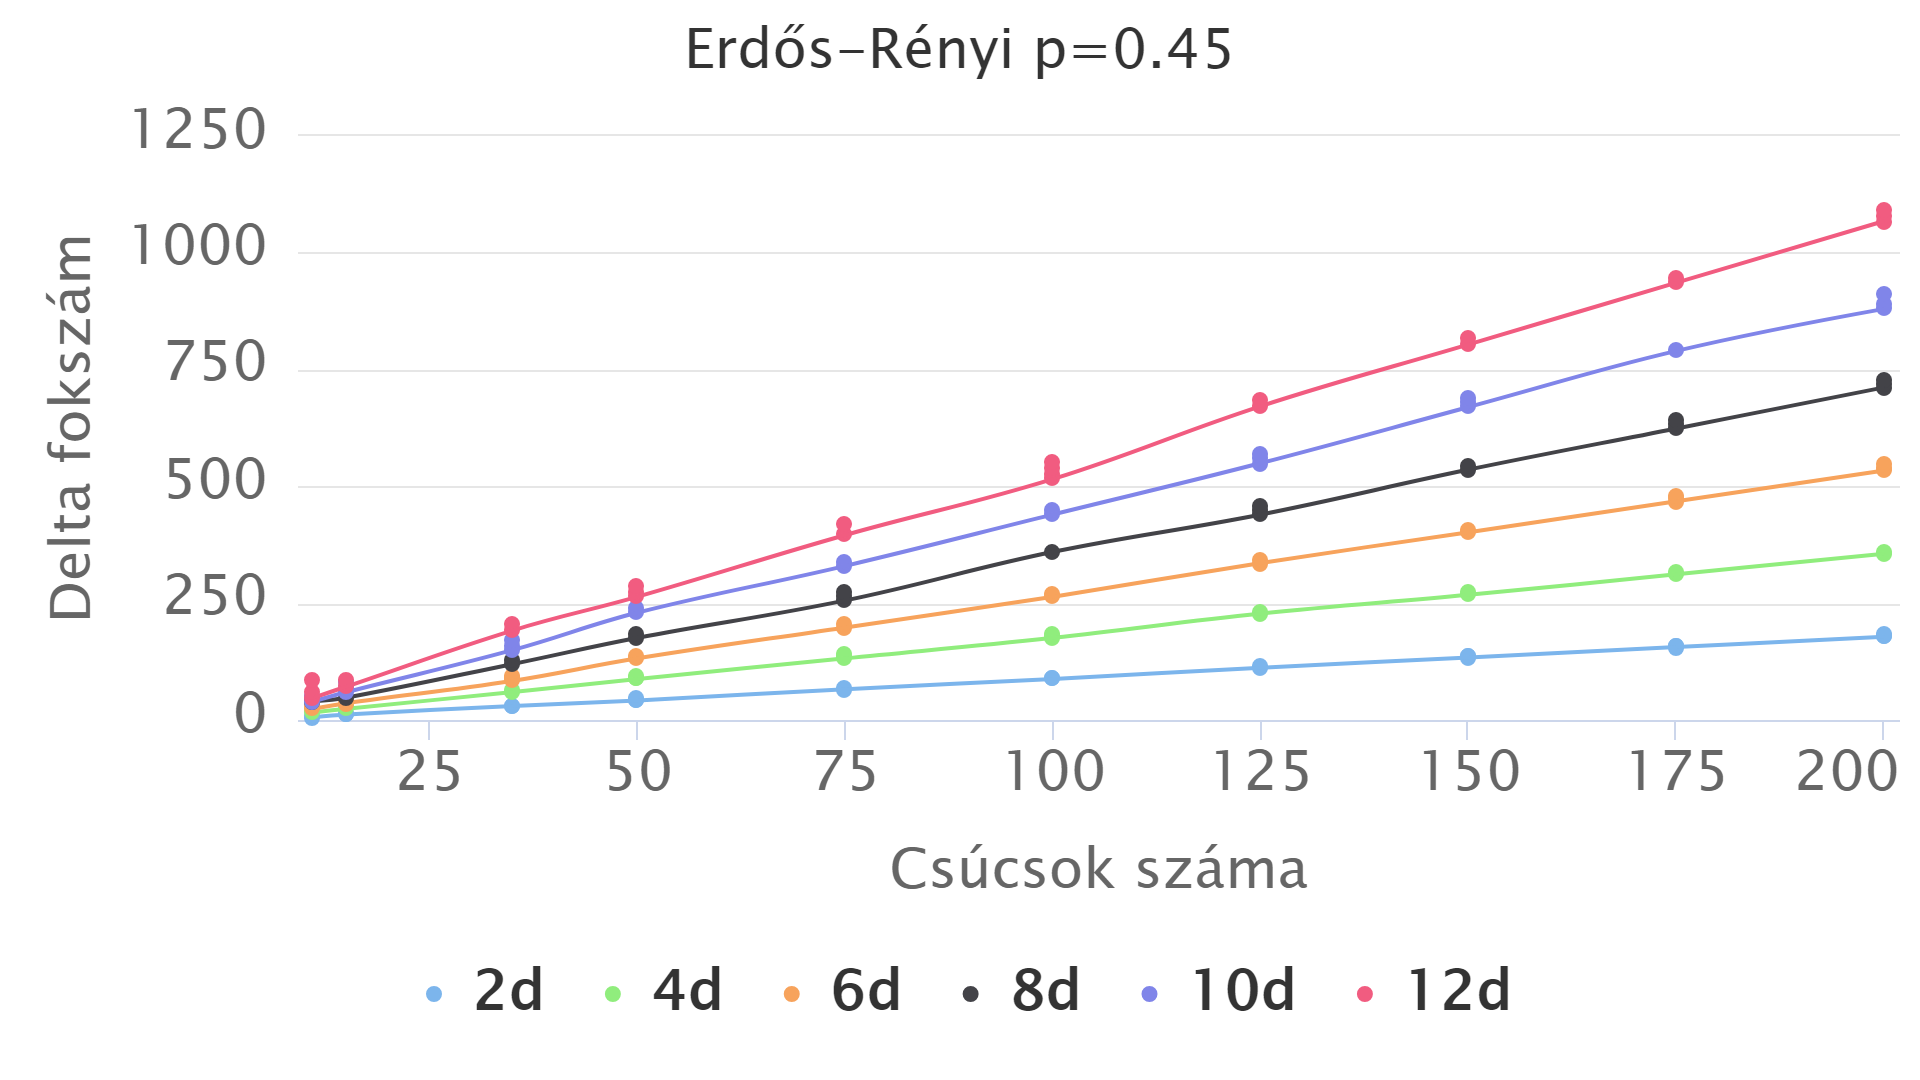
\includegraphics[width=0.49\linewidth]{pictures/constant_dan_ratio45_delta.png}
		\caption{Delta fokszám}
	\end{center}
\end{figure}

\begin{figure}[h]
	\begin{center}
		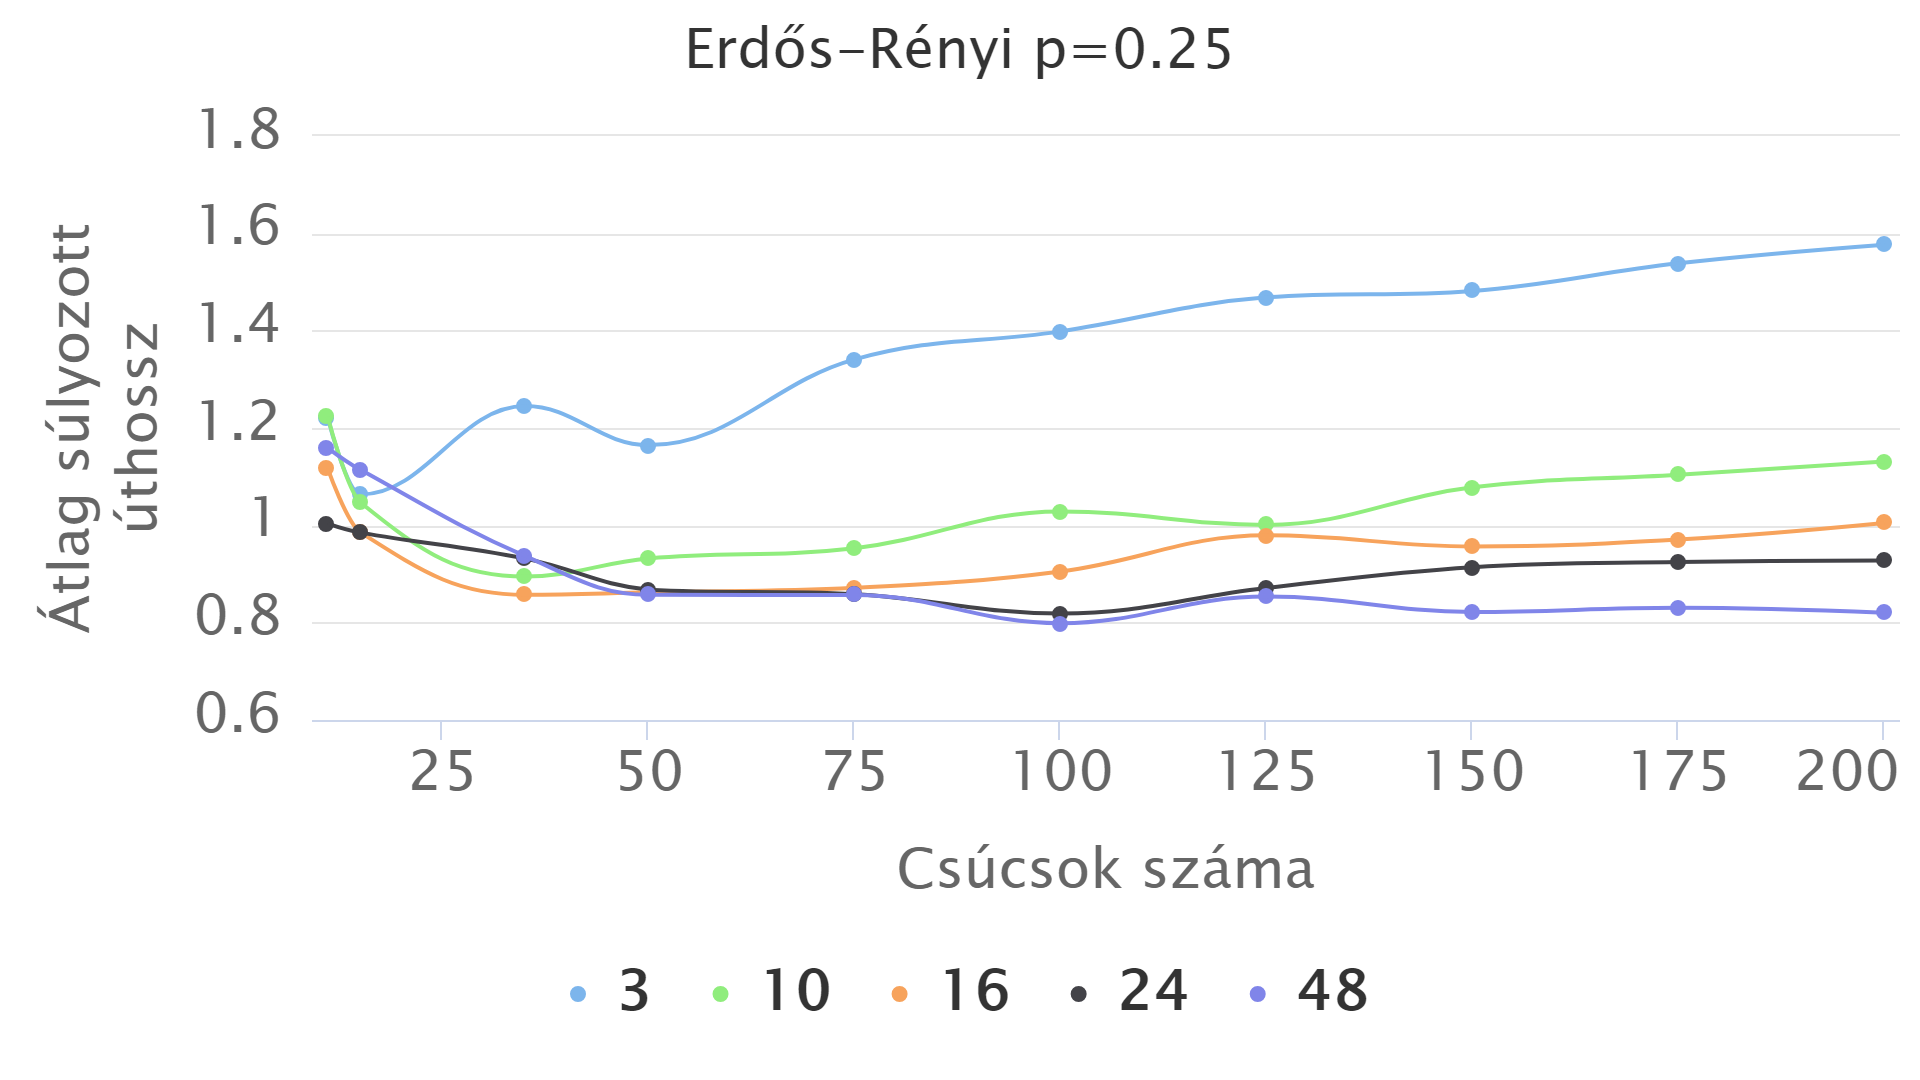
\includegraphics[width=0.49\linewidth]{pictures/constant_dan_ratio25_avg_route_len.png}
		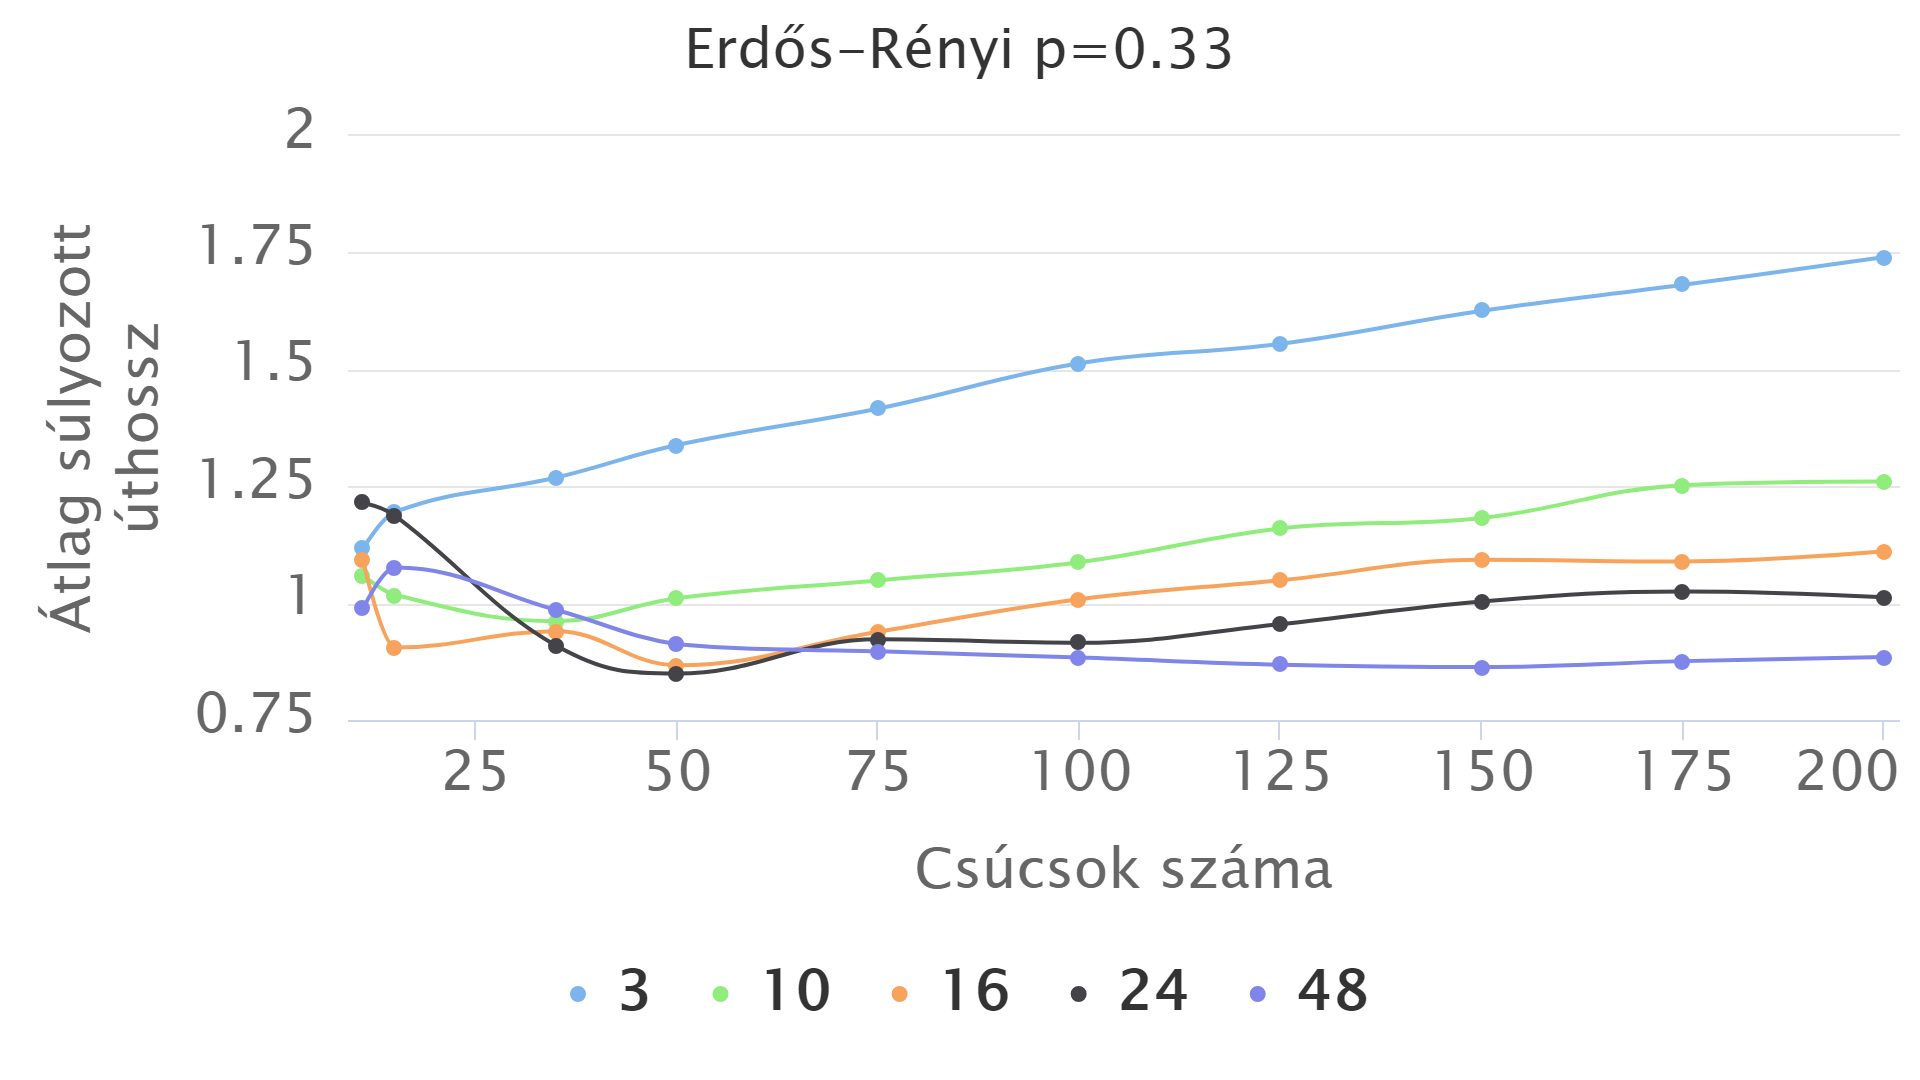
\includegraphics[width=0.49\linewidth]{pictures/constant_dan_ratio33_avg_route_len.png}
		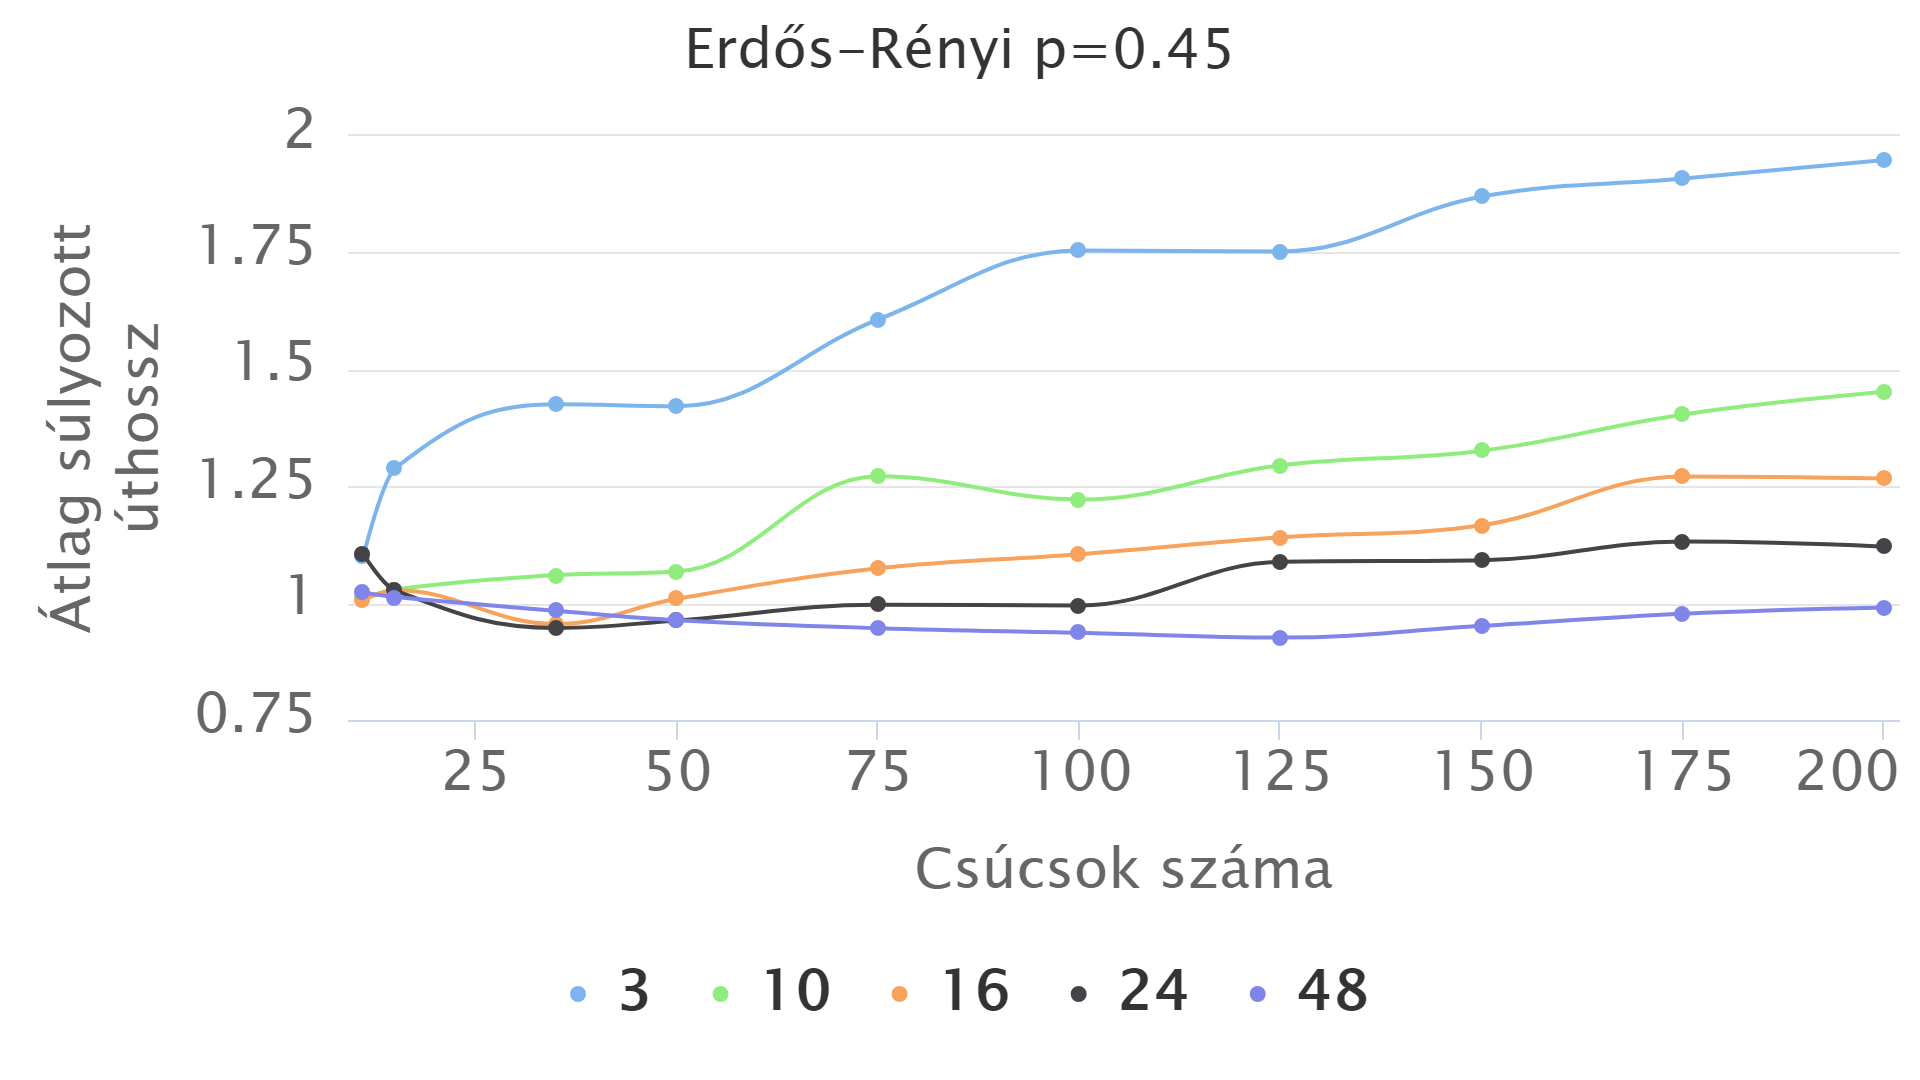
\includegraphics[width=0.49\linewidth]{pictures/constant_dan_ratio45_avg_route_len.png}
		\caption{Átlag súlyozott úthossz}
	\end{center}
\end{figure}

\begin{figure}[h]
	\begin{center}
		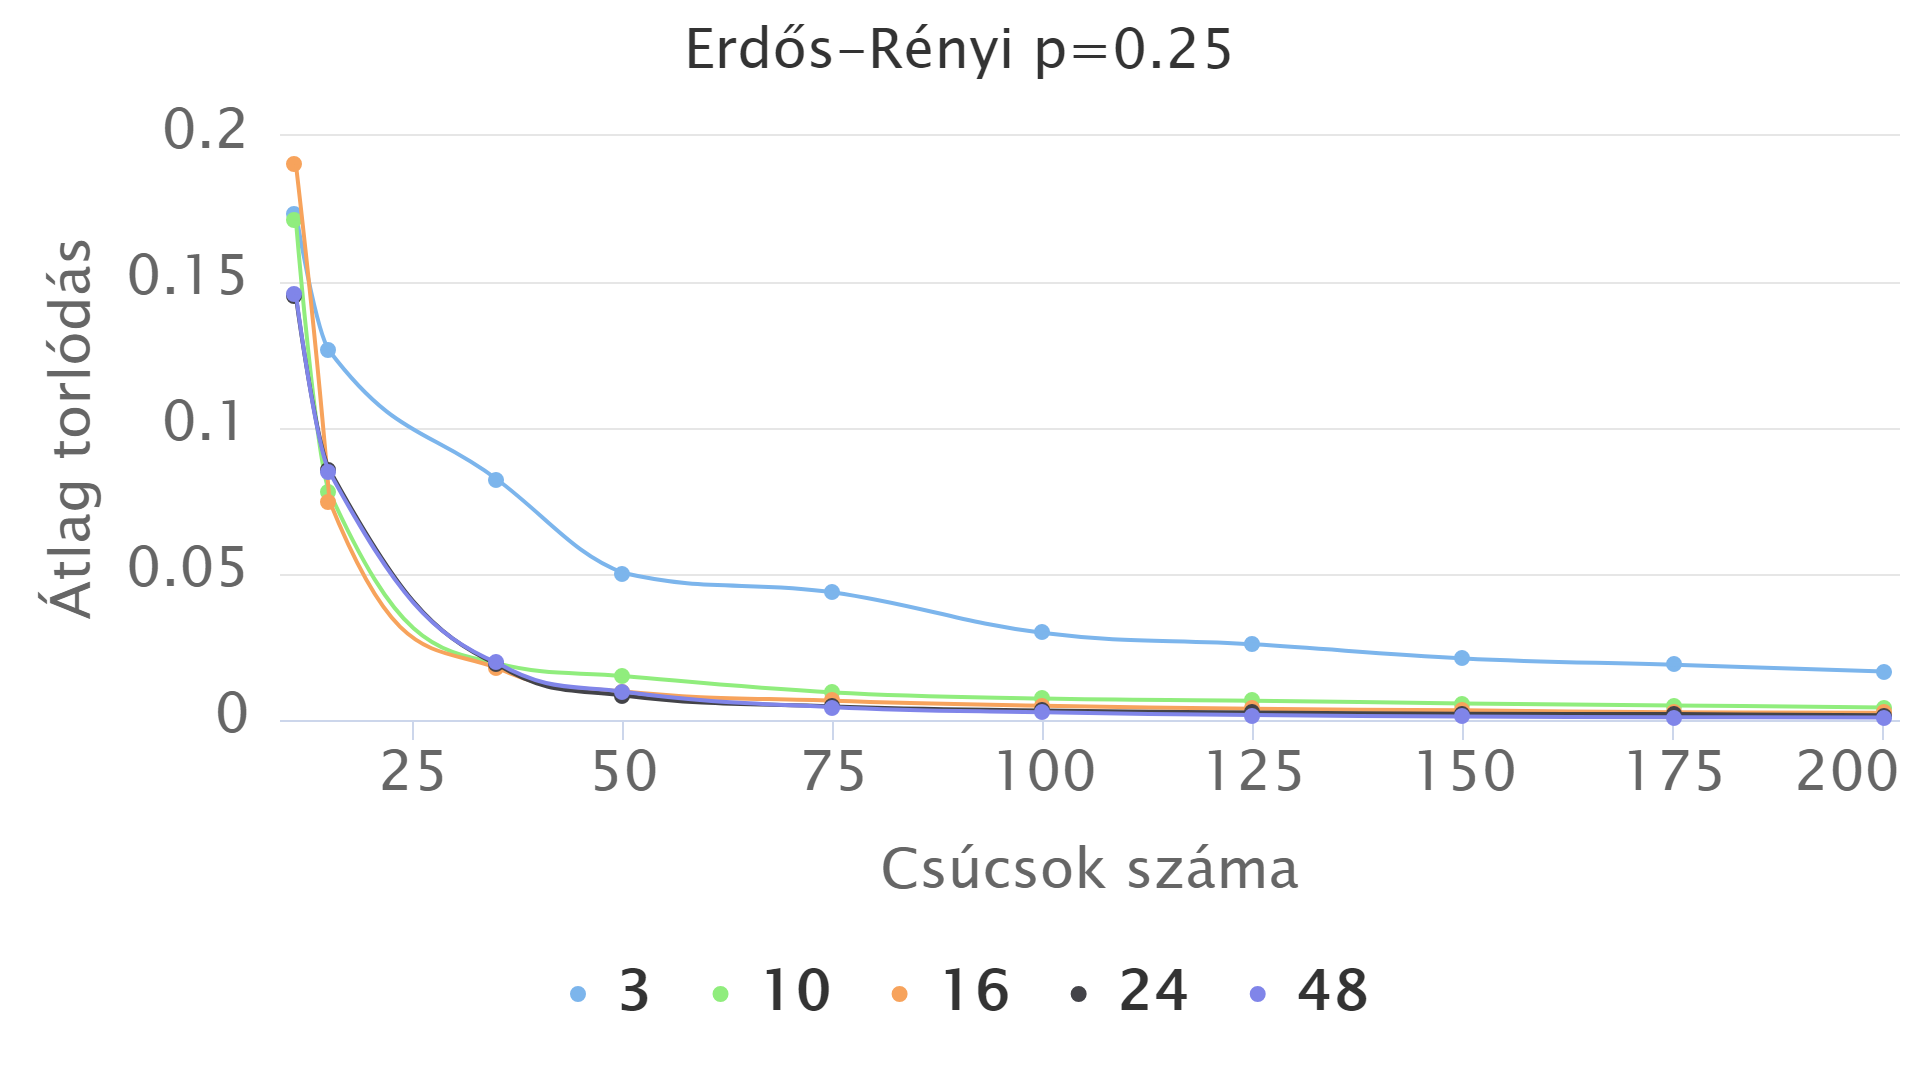
\includegraphics[width=0.49\linewidth]{pictures/constant_dan_ratio25_congestion.png}
		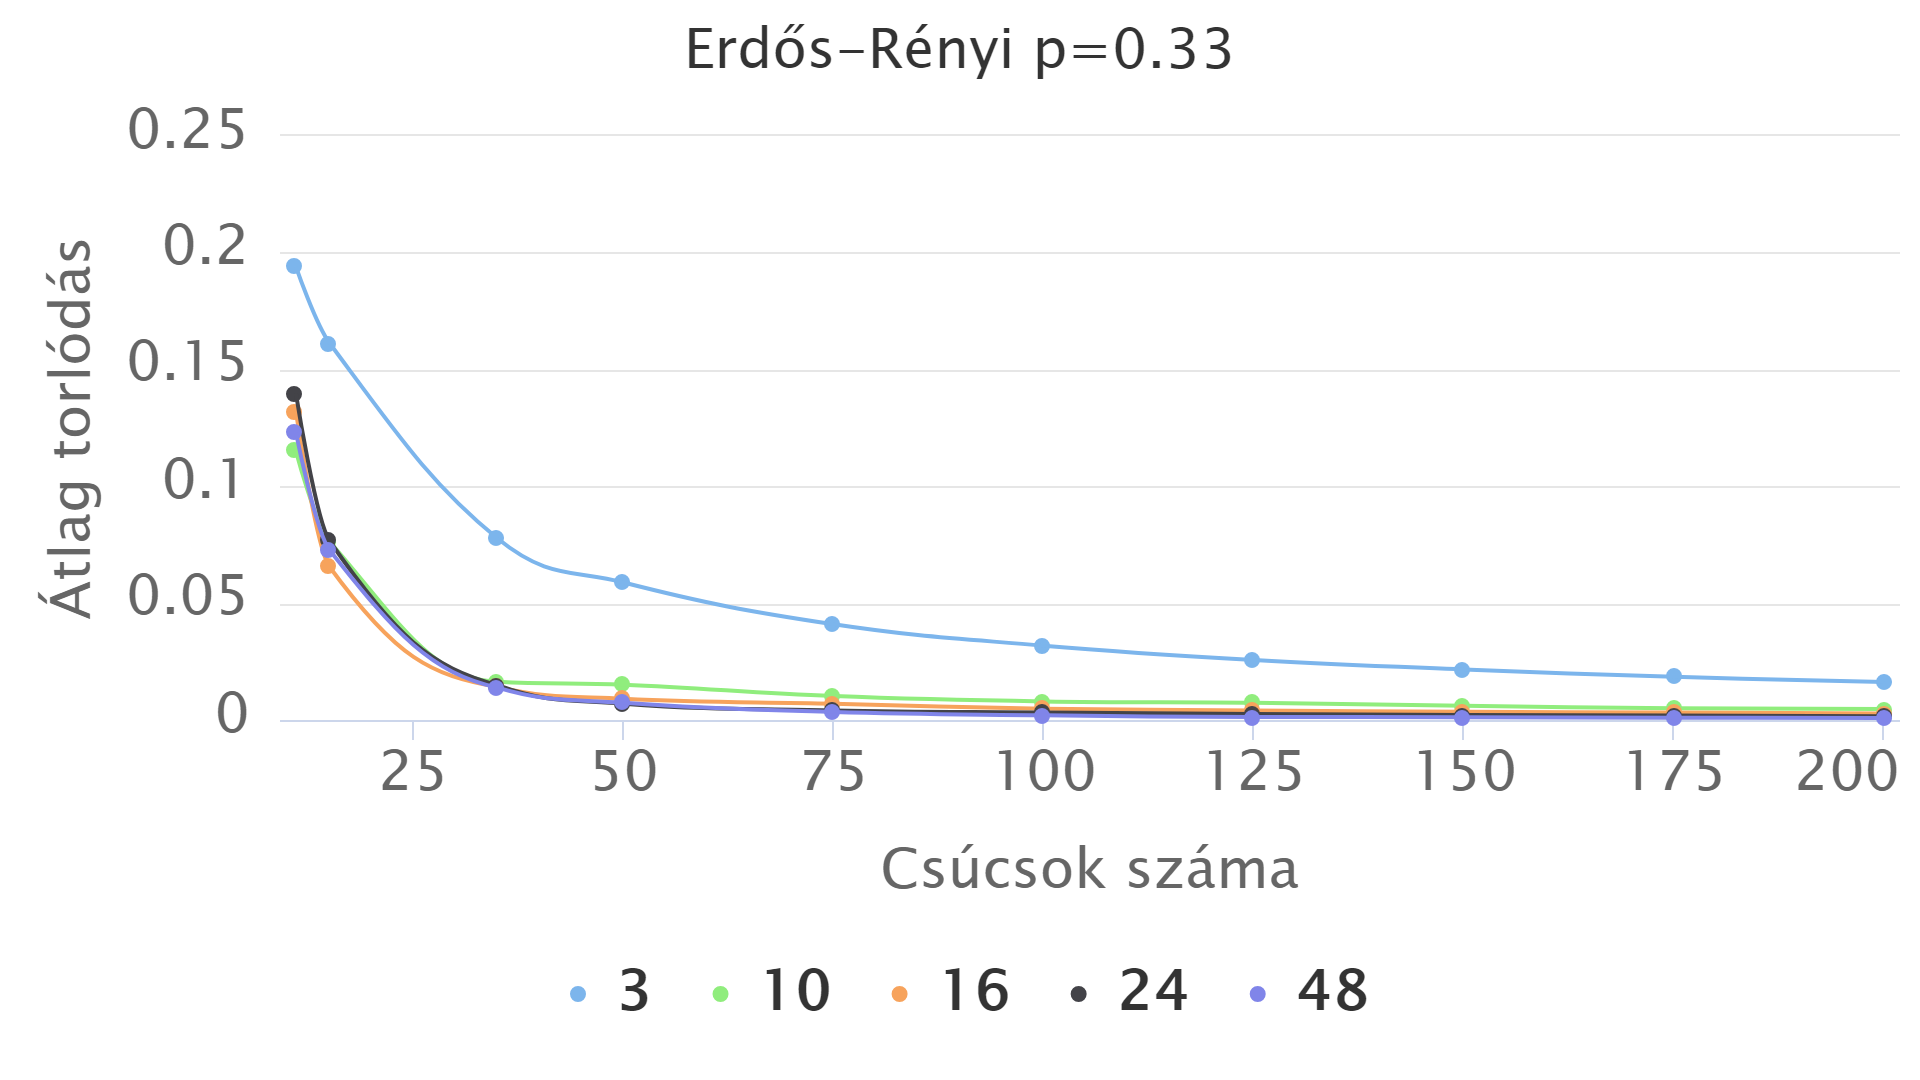
\includegraphics[width=0.49\linewidth]{pictures/constant_dan_ratio33_congestion.png}
		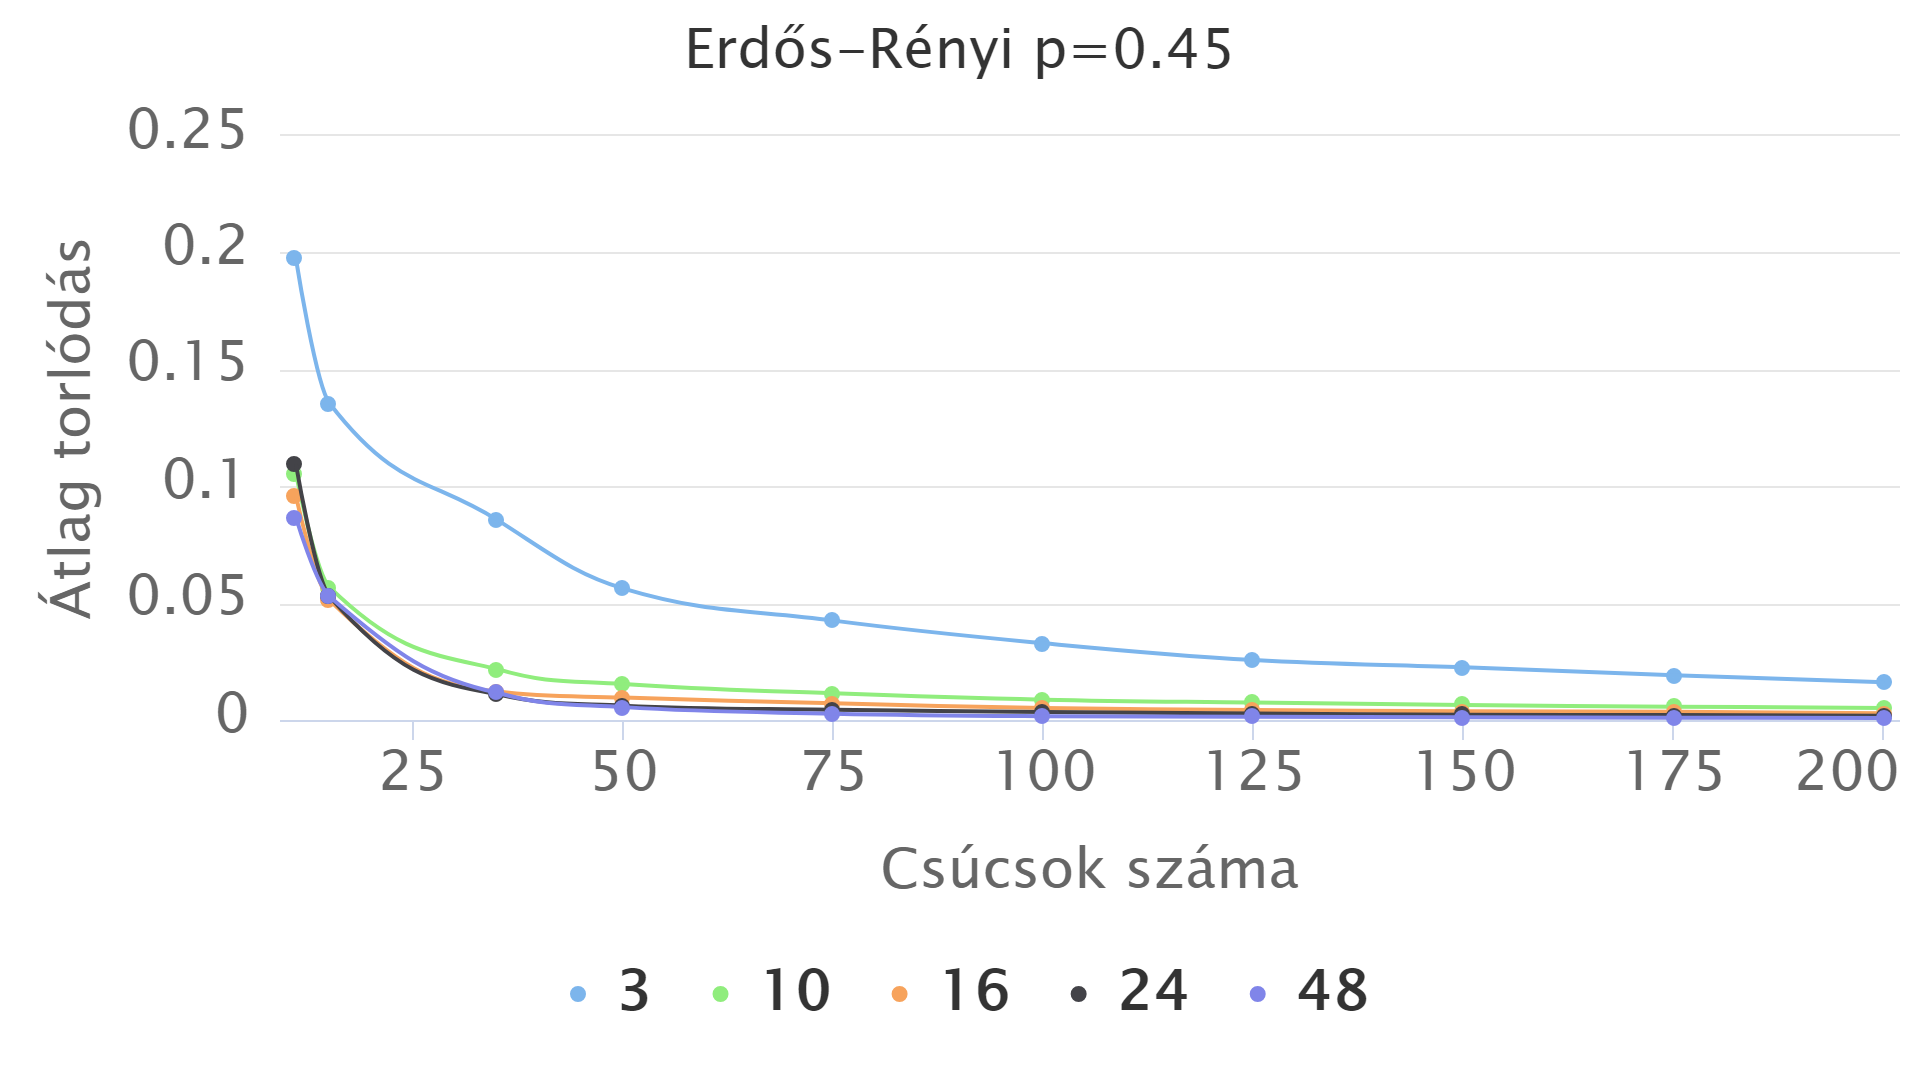
\includegraphics[width=0.49\linewidth]{pictures/constant_dan_ratio45_congestion.png}
		\caption{Átlag súlyozott úthossz}
	\end{center}
\end{figure}


\chapter{Összefoglalás}

\bibliographystyle{abbrv}
\bibliography{refrences}

	
\end{document}